\section{Waves}

Wave is a way of transferring and storing \emph{energy} without the transport of matter. Most familiar examples are surface waves on water, sound waves, light waves. In the next two chapters, we are going to look at the basics of wave motion and some of the most important wave phenomena.

%Wave motion is the propagation of disturbance -- deviations from a state of equilibrium -- from one place to another. 
%
%Waves consist of continuous oscillations around some fixed locations.
%
%There are mainly two types of waves, \keypoint{mechanical waves} and \keypoint{electromagnetic waves}. Mechanical waves propagate as oscillations of matter, thus it must travel through a \emph{medium}. Electromagnetic waves can travel in free space.
%
%A wave can either be \keypoint{transverse} or \keypoint{longitudinal} depending on the direction of its oscillation. The direction of propagation of a transverse wave is perpendicular to the direction of its oscillation, and the wave motion of a longitudinal wave is parallel to its oscillation.

\subsection{wave terminologies}

wave motion is the propagation of disturbance from one place to another

\begin{figure}[ht]
	\centering
	\begin{tikzpicture}[xscale=1.2, yscale=0.95]
	\draw [->] (0,-2) -- (0,2.4) node[midway,left]{$O$} node[above]{displacement};
	\draw [->] (0,0) -- (3.1*pi,0) node[below]{position};
	\draw[very thick,->] (1.8*pi,2) -- (2.6*pi,2);
	\node[above,twoline] at (2.2*pi, 2.1) {direction of\\wave motion};
	\foreach \t/\labelcolor in {1/{blue}, 2/{Green}, 3/{purple}, 4/{gray}} {
		\draw[\labelcolor] ({0.4*pi+(\t-1)*0.6)}, 1.7) --++ (0.2,0.5) node[above]{$t_\t$};
		\draw [thick, \labelcolor, domain=0:3*pi, samples=30, smooth] plot (\x,{1.6*sin((\x+0.6-0.6*\t)*1.25 r)});
	}
	\end{tikzpicture}
	
	\caption*{wave pattern at different times ($t_1<t_2<t_3<t_4$) as wave travels in space}
\end{figure}


to describe the wave motion and particle vibrations, we can define the following quantities:


\cmt as a wave moves out, each point oscillates back and forth about their rest positions

distance from a particle's equilibrium position is called \keypoint{displacement} of the particle \index{displacement}

\cmt greatest displacement for a particle is called the \keypoint{amplitude} ($A$) \index{amplitude}

\cmt wave pattern repeats itself over a certain distance

distance between two adjacent points undergoing exactly same motion is the \keypoint{wavelength} ($\lambda$) \index{wavelength}

one can think of wavelength as crest-to-crest distance, trough-to-trough distance, etc.\footnote{For now, we take for granted that a wave is transverse. There are also longitudinal waves for which terms like crest and trough do not apply. We will get into that in \S\ref{ch-Lwaves}.}

\cmt each point also repeats its vibrational motion over a certain time interval

time for a particle to complete a full oscillation cycle is the  \keypoint{period} ($T$) \index{period}

\cmt number of oscillations for a particle per unit time is the \keypoint{frequency} ($f$) \index{frequency}

frequency can also be defined as the number of crests passing a given point per unit time

frequency of a wave is related to its period by $\boxed{f=\frac{1}{T}}$

unit of frequency: $[f] = \text{Hz}$ (hertz), where $1 \text{ Hz} = 1 \text{ s}^{-1}$

\begin{figure}[ht]
	\centering
	\begin{minipage}{0.48\textwidth}
		\centering
		\begin{tikzpicture}[scale=0.55]
		\draw [->] (0,-2) -- (0,2) node[midway,left]{$O$} node[above]{displacement};
		\draw [->] (0,0) -- (3*pi,0) node[below]{position};
		\draw [very thick,blue,domain=0:3*pi,samples=30,smooth,variable=\x] plot (\x,{1.6*sin(\x*1.25 r)});
		\draw[<->, thick, red] (.4*pi,1.6) -- (.4*pi,0) node[midway,right]{$A$};
		\draw[<->, thick, red] (.4*pi,1.8) -- (2*pi,1.8) node[midway,above]{$\lambda$};
		\end{tikzpicture}
		
		wave pattern of all particles at one instant
	\end{minipage}\hfil
	\begin{minipage}{0.48\textwidth}
		\centering
		\begin{tikzpicture}[scale=0.55]
		\draw [->] (0,-2) -- (0,2) node[midway,left]{$O$} node[above]{displacement};
		\draw [->] (0,0) -- (3*pi,0) node[below]{time};
		\draw [very thick,blue,domain=0:3*pi,samples=30,smooth,variable=\x] plot (\x,{1.6*sin(\x*1.25 r)});
		\draw[<->, thick, red] (.4*pi,1.6) -- (.4*pi,0) node[midway,right]{$A$};
		\draw[<->, thick, red] (.4*pi,1.8) -- (2*pi,1.8) node[midway,above]{$T$};
		\end{tikzpicture}
		
		vibration of one specific particle at all times
	\end{minipage}
\end{figure}

\cmt wave energy is transferred along the direction of wave motion at a certain speed $v$

in one period, wave moves forward by a distance of one wavelength

so \keypoint{wave speed} $\boxed{v=\frac{\lambda}{T}}$, or in terms of frequency, $\boxed{v=\lambda f}$

\example{When a wave travels on a water surface, the maximum depth of water is 21 cm and the minimum depth is 18 cm. What is the amplitude of the wave?}

\sol amplitude is half the end-to-end distance: $ A = \frac{1}{2}(21-18) = 1.5 \text{ cm} $ \eoe


\example{A wave travelling at $4.0 \mps$ has a wavelength of 50 cm, what is its period?}

\solc\begin{equation*}
	v = \frac{\lambda}{T} \RA T = \frac{\lambda}{v} = \frac{0.50}{4.0} = 0.125 \text{ s} \teoe
\end{equation*}








\subsection{transverse \& longitudinal waves}

a wave can either be \emph{transverse} or \emph{longitudinal}, depending on the direction of its oscillation

\subsubsection{transverse waves}

\begin{ilight}
	\centering a \keypoint{transverse} wave has vibrations at right angle to its direction of energy transfer \index{transverse wave}
\end{ilight}

\cmt examples of transverse waves: wave on a string, surface wave on water, light wave, etc.

\cmt for a transverse wave, greatest displacement in positive direction is called a \emph{crest}, or a \emph{peak}

greatest displacement in negative direction is called a \emph{trough}


\subsubsection{longitudinal waves} \label{ch-Lwaves}

\begin{ilight}
	\centering a \keypoint{longitudinal} wave has vibrations in parallel direction to energy transfer \index{longitudinal wave}
\end{ilight}

\cmt examples of longitudinal waves: sound waves, wave along a stretched slinky, etc.

\cmt for a longitudinal wave, if medium gets squeezed, we say this region is a \emph{compression}

if a medium expands, we say this region is a \emph{rarefaction}

\cmt wavelength of a longitudinal wave can be defined as compression-to-compression distance

\begin{figure}[ht]
	\centering
	\begin{tikzpicture}[xscale=1, yscale=1.7]
	\foreach \x in {-0.75,-0.5,...,10.75}
	\draw[thick] ({\x} , -1) --++ (0,1);
	\end{tikzpicture}
	
	all particles at their equilibrium position before a pressure wave is set up
\end{figure}

\begin{figure}[ht]
	\centering
	\begin{tikzpicture}[xscale=1, yscale=1.7]
	\foreach \x in {-0.75,-0.5,...,11} 
		\draw[thick] ({\x+0.5*cos(\x*0.5*pi r)} , -1) --++ (0,1);
	\foreach \x in {-0.5,-0.25,...,11.25} 
		\draw[thick] ({\x+0.5*cos((\x-1)*0.5*pi r)} , -2.5) --++ (0,1);
	\foreach \x in {-0.5,-0.25,...,11} 
		\draw[thick] ({\x+0.5*cos((\x-2)*0.5*pi r)} , -4) --++ (0,1);
		\foreach \x in {3,7} \node[Green] at (\x,-1.2) {\phantom{p}rarefaction\phantom{p}};
		\foreach \x in {1,5,9} \node[blue] at (\x,-1.2) {compression};
		\foreach \x in {0,4,8} \node[Green] at (\x,-2.7) {\phantom{p}rarefaction\phantom{p}};
		\foreach \x in {2,6,10} \node[blue] at (\x,-2.7) {compression};
		\foreach \x in {1,5,9} \node[Green] at (\x,-4.2) {\phantom{p}rarefaction\phantom{p}};
		\foreach \x in {3,7} \node[blue] at (\x,-4.2) {compression};
		\node at (-1.5,-0.5) {{\large $t_1$}};
		\node at (-1.5,-2) {{\large $t_2$}};
		\node at (-1.5,-3.5) {{\large $t_3$}};
		\draw[very thick,->] (2.8,0.3) -- (7.2,0.3);
		\node[above,twoline] at (5, 0.4) {direction of wave motion};
		\draw[thick,red,<->] (1,-0.5) -- (5,-0.5) node[above,pos=0.55]{$\lambda$};
	\end{tikzpicture}
	
	compression and rarefaction regions at different times ($t_1<t_2<t_3$)
	
	as a longitudinal pressure wave travels in space
\end{figure}



\example{What is the distance between a compression and a rarefaction for a sound wave of frequency 550 Hz? (Speed of sound in air is about $330 \mps$.)}

\solc\begin{equation*}
	d = \frac{1}{2}\lambda = \frac{v}{2f} = \frac{330}{2\times 550} \RA d = 0.30 \text{ m} \teoe
\end{equation*}


\subsubsection{sound waves}

sound waves propagate via the compression and rarefaction of air (or other medium) \index{sound}

molecules near vibrating source is pushed away from rest positions and into their neighbours

neighbouring molecules then in turn push into their neighbours, and so on

the disturbance is transferred through the medium, forming a sound wave

\cmt sound waves are longitudinal
	
\begin{figure}[htp]
\centering
	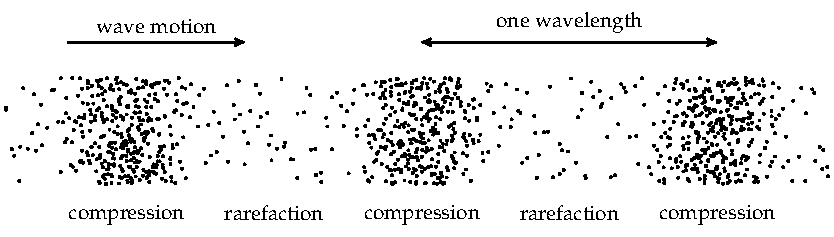
\includegraphics[width=0.95\textwidth]{longitudinal.pdf}
	\caption*{disturbance of vibrating molecules in a sound wave}
\end{figure}

\cmt propagation of sound waves require medium (air, water, steel, etc.)
	
sound cannot travel in vacuum
	
\cmt speed of sound is material-dependent, but not frequency-dependent
	
	sound in general travels faster in denser medium
	
	\titem $v_\text{air} \approx 340 \mps$ (under standard atmospheric pressure and room temperature)
	
	\titem $v_\text{water} \approx 1500 \mps$
	
	\titem $v_\text{steel} \approx 5000 \mps$
	
\cmt \emph{pitch} of a note is related to frequency of sound wave

rapid vibrations of sound source at high frequencies produce a high pitch

\cmt \emph{loudness} of sound mainly depends on amplitude of vibration

a greater amplitude means the wave is more energetic so it sounds louder
	

\subsubsection*{measurement of sound waves}

two key apparatuses for sound measurement are the \keypoint{microphone} and the \keypoint{oscilloscope} \index{oscilloscope}

sound waves can be captured by a \emph{microphone}, which converts sound into electrical signals

electrical signals can then be sent into an \emph{oscilloscope} (see figure\footnote{The beautiful figure of the oscilloscope was created by \emph{Hugues Vermeiren}, who generously shared the source codes on TeXample: \url{http://www.texample.net/tikz/examples/textronics-oscilloscope/}}) for measurement

oscilloscope can be thought as an upgraded voltmeter showing how voltage varies with time

\begin{figure}[ht]
	\centering
	\includegraphics*[width=0.88\textwidth]{oscilloscope.pdf}
	
	the display and controls of a typical cathode-ray oscilloscope
\end{figure}

\cmt oscilloscope displays the variation of voltage ($y$-axis) with time ($x$-axis)

\cmt horizontal scale (time axis) is given by \emph{time-base} settings

vertical scale (voltage axis) is given by \emph{voltage gain}, or \emph{Y-sensitivity} settings

\cmt period $T$ of the sound wave can be found using time-base settings

then frequency of sound wave is calculated: $f=\frac{1}{T}$

\cmt voltage amplitude can be found using the voltage gain


\begin{wrapfigure}{r}{0.45\textwidth}
	\vspace*{-12pt}
	\centering
	\begin{tikzpicture}[scale=0.8]
	\draw[fill=gray!80, rounded corners] (-0.2,-3.2) rectangle (7.2,3.2);
	\draw[Green!50, fill] (0,-3) rectangle (7,3);
	\draw[Green!20, ultra thick, domain=0:7, samples=100] plot (\x, {2*sin((\x-0.6)*120)});
	\draw[black!80, step=1] (0,-3) grid (7,3);
	\end{tikzpicture}
	\vspace*{-16pt}
\end{wrapfigure}

\example{A sound wave is detected by a microphone and the trace is displayed on an oscilloscope as shown. If the time-base is set at 0.5 ms div$^{-1}$ and the voltage gain is set at 2 V div$^{-1}$. What is the frequency and the amplitude of the signal?}

\sol period: $T = 3 \times 0.5 \text{ ms} = 1.5 \times10^{-3} \text{ s}$

\eqyskip frequency: $f = \frac{1}{T} = \frac{1}{1.5 \times10^{-3} \text{ s}} \approx 667 \text{ Hz}$

\eqyskip amplitude: $A = 2 \times 2 \text{ V} = 4.0 \text{ V}$ \eoe




\subsection{electromagnetic waves}

a wave can be either \emph{mechanical} or \emph{electromagnetic}, depending on whether it requires a medium\index{electromagnetic wave}

\cmt waves that require a \emph{medium} to travel are called \keypoint{mechanical waves}

examples are sound waves, water waves, wave on a string, etc.

mechanical waves involve vibration of matter particles

\cmt no medium is needed for propagation of \keypoint{electromagnetic waves} i.e., they can travel in vacuum



\subsubsection{properties of electromagnetic waves}

\cmt electromagnetic waves can travel in free space

\cmt electromagnetic waves involve vibrations of electric and magnetic fields
	
an altering electric field can generate an altering magnetic field, which then further produces a new altering electric field, so on and so forth

electric and magnetic fields then permeate through space, transferring energy and information
	
\cmt electromagnetic waves are all transverse
	
vibration of electric fields and magnetic fields are both perpendicular to wave motion

\begin{figure}[ht]
	\centering
	\begin{tikzpicture}[xscale=0.72]
	\draw[Green, thick, ->] (0,-2.1) -- (0,2.1) node[left, twoline] {electric\\field};
	\draw[blue, thick, dotted] (0 ,0) -- (0.7, 1.4);
	\draw[blue, thick, ->] (0, 0) -- (-0.7,-1.4) node[left, twolinecap] {magnetic\\field};
	\draw[thick, ->] (-0.3,0) -- (14,0) node[right, twoline]{direction\\ of energy\\transfer};
	\draw[Green, thick, domain=0:13.5, samples=150] plot (\x, {1.6*sin(2*\x r)});
	\draw[blue, thick] plot [smooth] coordinates {
		(0, 0)
		(0.0007, -0.1987)
		(0.0053, -0.3894)
		(0.0177, -0.5646)
		(0.0413, -0.7174)
		(0.0793, -0.8415)
		(0.134, -0.932)
		(0.2073, -0.9854)
		(0.3002, -0.9996)
		(0.4131, -0.9738)
		(0.5454, -0.9093)
		(0.6958, -0.8085)
		(0.8623, -0.6755)
		(1.0422, -0.5155)
		(1.2325, -0.335)
		(1.4294, -0.1411)
		(1.6292, 0.0584)
		(1.8278, 0.2555)
		(2.0213, 0.4425)
		(2.2059, 0.6119)
		(2.3784, 0.7568)
		(2.5358, 0.8716)
		(2.6758, 0.9516)
		(2.7968, 0.9937)
		(2.8981, 0.9962)
		(2.9795, 0.9589)
		(3.0417, 0.8835)
		(3.0864, 0.7728)
		(3.1156, 0.6313)
		(3.1323, 0.4646)
		(3.1397, 0.2794)
		(3.1415, 0.0831)
		(3.1417, -0.1165)
		(3.1442, -0.3115)
		(3.1529, -0.4941)
		(3.1715, -0.657)
		(3.2032, -0.7937)
		(3.2506, -0.8987)
		(3.316, -0.9679)
		(3.4007, -0.9985)
		(3.5053, -0.9894)
		(3.6296, -0.9407)
		(3.7727, -0.8546)
		(3.9328, -0.7344)
		(4.1075, -0.5849)
		(4.2939, -0.4121)
		(4.4886, -0.2229)
		(4.6876, -0.0248)
		(4.8872, 0.1743)
		(5.0832, 0.3665)
		(5.272, 0.544)
		(5.4499, 0.6999)
		(5.6139, 0.8278)
		(5.7614, 0.9228)
		(5.8905, 0.9809)
		(6, 1)
		(6.0896, 0.9792)
		(6.1597, 0.9193)
		(6.2114, 0.8228)
		(6.2468, 0.6935)
		(6.2683, 0.5366)
		(6.2791, 0.3582)
		(6.2828, 0.1656)
		(6.2832, -0.0336)
		(6.2842, -0.2315)
		(6.2899, -0.4202)
		(6.304, -0.5921)
		(6.3298, -0.7404)
		(6.3704, -0.8592)
		(6.4282, -0.9437)
		(6.5047, -0.9906)
		(6.601, -0.998)
		(6.7172, -0.9657)
		(6.8526, -0.8948)
		(7.0059, -0.7883)
		(7.1749, -0.6503)
		(7.3568, -0.4864)
		(7.5484, -0.3031)
		(7.7461, -0.1078)
		(7.946, 0.0919)
		(8.144, 0.2879)
		(8.3362, 0.4724)
		(8.5191, 0.6381)
		(8.6892, 0.7784)
		(8.8438, 0.8876)
		(8.9807, 0.9614)
		(9.0985, 0.9969)
		(9.1963, 0.9927)
		(9.2744, 0.9488)
		(9.3336, 0.8672)
		(9.3755, 0.751)
		(9.4024, 0.6048)
		(9.4173, 0.4346)
		(9.4235, 0.247)
		(9.4248, 0.0495)
		(9.4251, -0.1499)
		(9.4283, -0.3433)
		(9.4385, -0.5231)
		(9.459, -0.682)
		(9.4932, -0.8137)
		(9.5435, -0.9129)
		(9.6121, -0.9758)
		(9.7001, -0.9998)
		(9.808, -0.9839)
		(9.9356, -0.9288)
		(10.0817, -0.8367)
		(10.2444, -0.7112)
		(10.4213, -0.5573)
		(10.6094, -0.3813)
		(10.805, -0.19)
		(11.0044, 0.0089)
		(11.2037, 0.2073)
		(11.3988, 0.3976)
		(11.586, 0.5719)
		(11.7617, 0.7235)
		(11.9231, 0.8462)
		(12.0676, 0.9352)
		(12.1935, 0.9869)
		(12.2996, 0.9993)
		(12.3859, 0.9718)
		(12.4528, 0.9056)
		(12.5016, 0.8033)
		(12.5345, 0.6689)
		(12.5539, 0.5079)
		(12.5633, 0.3266)
		(12.5662, 0.1324)
		(12.5664, -0.0672)
		(12.568, -0.2641)
		(12.5748, -0.4504)
		(12.5906, -0.6188)
		(12.6187, -0.7626)
		(12.6621, -0.8759)
		(12.7229, -0.9543)
		(12.8027, -0.9946)
		(12.9023, -0.9954)
		(13.0218, -0.9564)
		};
	\end{tikzpicture}
	\caption*{variation in electric and magnetic fields for an electromagnetic wave}
\end{figure}

	
\cmt all electromagnetic waves travel at a constant speed $c=3.0\times10^8\mps$ in free space

i.e., speed of light in vacuum is constant\footnote{The speed of light in vacuum is actually a \emph{universal} physical constant. According to Einstein's special relativity, this is the upper limit for the speed at which matter and information can travel. This speed is also independent of the inertial reference frame one chooses, i.e., the speed of light in vacuum is the same for all observers, regardless of the motion of the source or the observer.}



\subsubsection{electromagnetic spectrum}

electromagnetic waves come in a wide range of wavelengths and frequencies 

distribution of electromagnetic radiation according to wavelength or frequency is the \keypoint{electromagnetic spectrum}\index{electromagnetic spectrum} (see diagram)



\begin{figure}[!ht]
	\centering
	\begin{tikzpicture}[yscale=1.04]
	% define visible spectrum shading
	\pgfdeclareverticalshading{visible}{100bp}
	{color(0bp)=(violet!70); color(25bp)=(violet!70); color(35bp)=(blue!70);
		color(45bp)=(green!70); color(55bp)=(yellow!70); color(65bp)=(orange);
		color(75bp)=(red); color(100bp)=(red)}
	% grayish background for spectrum labels
	\draw[gray!15,fill] (-1.5,-8) rectangle (1.5,7.5);
	% axes
	\draw (-1.5,-8) -- (-1.5,7.5) (1.5,-8) -- (1.5,7.5);
	\node at (-3,7.7) {wavelength};
	\node at (3,7.7) {frequency};
	% spectrum labels
	\shade[shading=visible] (-1.5,-1.15) rectangle (1.5,-0.75);
	\foreach \x/\xlabel in {1.8/{radio waves}, -2/{microwaves}, -4.6/{infrared}, -6.35/{visible light}, -7.8/{ultraviolet}, -11/{X-rays}, -14.8/{$\gamma$-rays} } \node at (0,{\x*0.7+3.5}) {\xlabel};
	% values of wavelengths
	\foreach \x in {5,3,1,...,-15} {
		\draw (-1.5,{\x*0.7+3.5}) --++ (-0.5,0);
		\node at (-3,{\x*0.7+3.5}) {$10^{\x}$ m};
	}
	% values of frequencies
	\foreach \x in {3,5,...,23} {
		\draw (1.5,{-\x*0.7+8.8}) --++ (0.5,0);
		\node at (3,{-\x*0.7+8.8}) {$10^{\x}$ Hz};
	}
	% dashed lines as separators
	\foreach \x in {-1,-3,-9,-13} \draw[dashed,thick] (-1.5,{\x*0.7+3.5}) --++ (3,0);
	% extension for visible spectrum
	\draw[thick, gray!75] (1.5,-1.15) --++ (3,0) -- (5,-3);
	\draw[thick, gray!75] (1.5,-0.75) --++ (3,0) -- (5,1);
	\shade[shading=visible] (5,-3) rectangle (7,1);
	\node at (6, 1.3) {visible light};
	\node[right] at (7.2, 0.8) {700 nm};
	\node[right] at (7.2, -2.8) {400 nm};
	\end{tikzpicture}
	\caption*{the electromagnetic spectrum}
\end{figure}

\newpage

\cmt the table below shows electromagnetic spectrum in somewhat more precise details \footnote{There are no precise accepted boundaries between different ranges in the electromagnetic spectrum. The boundaries are actually somewhat ambiguous. The ranges of different portions tend to overlap. For example, a large portion of the ranges of X-rays overlap with that of $\gamma$-rays, and microwaves are considered by many people as a subdivision of radio waves. Therefore, the values given here are merely supposed to give you some rough idea about the order of magnitudes for electromagnetic wavelengths and frequencies. So the point I want to make here is: do not take the borderlines too seriously.}

\begin{center}
	\begin{tabular}{|C{4cm}|C{4cm}|C{4cm}|}
		\hline type of radiation & range of wavelength & range of frequency \\ 
		\hline radio waves  & 10$^{-1}$ $\sim$ 10$^{6}$ m & 10$^{2}$ $\sim$ 10$^{9}$ Hz \\ 
		\hline microwaves & 10$^{-3}$ $\sim$ 10$^{-1}$ m & 10$^{9}$ $\sim$ 10$^{11}$ Hz \\ 
		\hline infra-red & 7$\times$10$^{-7}$ $\sim$ 10$^{-3}$ m & 10$^{11}$ $\sim$ 10$^{14}$ Hz \\ 
		\hline visible light  & 4$\times$10$^{-7}$ $\sim$ 7$\times$10$^{-7}$ m & 10$^{14}$ $\sim$ 10$^{15}$ Hz \\ 
		\hline ultraviolet & 10$^{-9}$ $\sim$ 4$\times$10$^{-7}$ m & 10$^{15}$ $\sim$ 10$^{17}$ Hz \\ 
		\hline X-rays & 10$^{-13}$ $\sim$ 10$^{-9}$ m & 10$^{17}$ $\sim$ 10$^{19}$ Hz \\ 
		\hline $\gamma$-rays & 10$^{-16}$ $\sim$ 10$^{-11}$ m & 10$^{19}$ $\sim$ 10$^{24}$ Hz\\ 
		\hline
	\end{tabular} 
\end{center}

\cmt each type of electromagnetic waves has important applications in some area
\footnote{The entries listed here only include a teeny-weeny part of the uses of electromagnetic radiation, somewhat based on my personal taste. I also included a handful of explanations for the examples that I found interesting (otherwise I would not choose them), as you will see a huge load of footnotes in the next few pages. You are encouraged to do some researches as well, I can guarantee that you will not be disappointed.}

\begin{compactitem}
	\item[--] radio waves
	
	\xskip telecommunication (TV/radio broadcast, satellite communication) \footnote{Having the longest wavelengths of all radiation, radio waves have the best ability to diffract around obstacles in city buildings and mountains, therefore a large area can be covered.}

	\item[--] microwaves
	
	\xskip telecommunication (mobile phones, WiFi, Bluetooth, satellite communication)
	\footnote{Microwaves do not diffract sufficiently as radio waves, but they can transmit more information per unit time because they have higher frequencies. Microwaves are used in short-range telecommunication, including mobile phones, wireless networks, and bluetooth connections.}
		
		
	\xskip heating food (microwave ovens)
	\footnote{Frequency of microwaves are close to the natural frequencies of the rotational motion of water molecules. When food is exposed to microwaves, the water molecules in the food resonate and vibrate more violently, causing a rise in the food's temperature.}
	
	\item[--] infrared (IR)
	
	\xskip IR thermography (temperature monitors, thermographic cameras)
	\footnote{All objects emit electromagnetic radiation based on their temperatures. According to the law of black-body radiation, objects near room temperature emit thermal energy as infrared radiation, so variations in the temperature can be detected.}
	
	\xskip night-vision devices
	\footnote{Night-vision devices convert photons (just think of them as particles of light for now) into electrons, which are amplified by a chemical and electrical process and then converted back into visible light. Infrared sources can be used to augment the available light, increasing the visibility in the dark.}
	
	\xskip IR heating (IR heat lamps, IR saunas)
	
	
	\xskip IR data transmission (remote controls, optical-fibre communication)
	
	\item[--] visible light
	
	\xskip human vision
	\footnote{Human eyes are only sensitive to a small fraction of the electromagnetic spectrum. The wide variety of colours that we see is actually built up from the relative intensities of red, green and blue light collected by the three colour detectors in our eyes.}
	
	\item[--] ultraviolet (UV)
	
	\xskip UV sterilising (drinking water treatment, disinfection of medical facilities, etc.)
	\footnote{Short-wavelength UV light can damage the DNA's in living organisms. A microorganism exposed to germicidal UV light might not be able to reproduce, and becomes harmless. For the same reason, overexposure to UV radiation present in the sunlight can cause sunburn, or even skin cancer.}
		
	\xskip fluorescent dyes (black light fluorescent paint, UV watermarks)
	\footnote{UV radiation can cause many substances to glow through chemical reactions. UV watermarks that are visible under UV light are used to prevent counterfeiting of currency, or forgery of important documents such as passports and ID cards.}
	
	\item[--] X-rays
	
	\xskip medical imaging (X-ray imaging, CT scans)
	\footnote{X-rays are very energetic and thus very penetrating. They can pass through human body easily to form an image giving information about the structures of tissues and bones.}
	
	\xskip security check (luggage scanners)
	
	\xskip X-ray crystallography
	\footnote{X-rays can be diffracted by the lattice of atoms in a crystal. The diffraction pattern gives information about the structure of the lattice. X-ray crystallography is a very important experimental technique to study the microscopic structures of new materials.}
	
	\item[--] $\gamma$-rays
	
	\xskip radiation therapies (cancer treatment)
	\footnote{$\gamma$-rays have extremely high frequencies. They are even more energetic and penetrating. They can be used to damage the DNA of cancerous tissue, and hence kill the cancerous cells as a treatment.}
	
	\xskip medical imaging (PET scans)
	\footnote{Positron emission tomography (PET) uses a radioactive tracer to produce $\gamma$-rays within the tissues of interest. The energy and location of these $\gamma$-rays can be detected and sent to a computer to build up a 3D image of the body part.}
\end{compactitem}

\example{A beam of electromagnetic radiation is known to have a frequency of 25 THz in vacuum. What is its wavelength?}

\solc\begin{equation*}
	\lambda = \frac{c}{f} = \frac{3.00\times10^8}{25\times10^12} \RA \lambda = 1.2 \times 10^{-5} \text{ m} \quad \text{(infra-red)} \teoe
\end{equation*}


	

\subsection{wave intensity}

energy can be transmitted along a wave

the degree to which energy is concentrated is called the intensity of the wave

here concentration has two meanings -- concentration in time and concentration in area $S$\footnote{To avoid confusion, I reserved letter `$A$' for wave amplitude and chose `$S$' to represent an area.}

\begin{ilight}
	\centering \keypoint{intensity} of a wave is defined as the power $P$ per unit area on a cross section $S$: $\boxed{I=\frac{P}{S}}$ \index{wave intensity}
\end{ilight}

\cmt unit of wave intensity: $[I] = \text{ W m}^{-2}$

\cmt intensity is proportional to square of its amplitude: $\boxed{I \propto A^2}$.

\cmt intensity of a wave decreases as it spreads out in space

intensity at distance of $r$ from a point source is inversely proportional to $r^2$: $\boxed{I \propto \frac{1}{r^2}}$
\footnote{As a wave produced from a point source travels out by a distance $r$ away from the source, the energy it carries is spread uniformly over the surface area of the sphere of radius $r$, that is: $S=4\pi r^2$. So the intensity of a wave obeys an inverse square law: $I \propto \frac{1}{r^2}$.}

\example{If the amplitude of an incoming wave is increased by 50\%, what is the increase in the wave intensity?}

\sol $I \propto A^2 \RA \frac{I'}{I} = \left( \frac{A'}{A} \right)^2 = \left( 1 + 50\% \right)^2 =2.25 \RA $ so intensity is increased by 125\% \eoe

\newpage


\example{Two observers $A$ and $B$ are at a distance $r_A$ and $r_B$ from a point source where $r_A=2r_B$. (a) Find the ratio of their intensities $\frac{I_A}{I_B}$. (b) Find the ratio of their amplitudes $\frac{A_A}{B_B}$.}

\vspace*{0.8em}\solc

{
	\centering
	
	$ I \propto \frac{1}{r^2} \RA \frac{I_A}{I_B} = \left(\frac{r_B}{r_A}\right)^2 = \left(\frac{1}{2}\right)^2 \RA \frac{I_A}{I_B} = \frac{1}{4} $
	
	\vspace*{0.4em} $ I \propto A^2 \RA \frac{A_A}{A_B} = \sqrt{\frac{I_A}{I_B}} = \sqrt{\frac{1}{4}} \RA \frac{A_A}{A_B} = \frac{1}{2} $
	
}

\feoe




\subsection{polarisation}

\subsubsection{plane polarisation}

\begin{ilight}
	a wave is \keypoint{plane-polarised}, or simply \keypoint{polarised}, if the vibration is in one single direction at right angle to the direction of propagation of energy\index{polarisation}
\end{ilight}

\begin{figure}[ht]
	\centering
	\begin{minipage}{0.45\textwidth}
		\centering
		\begin{tikzpicture}[scale=0.6]
		\draw[very thick, blue, ->] (210:2) -- (30:8) node[twoline, above, black]{direction of\\energy transfer};
		\foreach \t in {0,45,90,135} {
			\draw[red, ultra thick, <->] (\t:1.5) --++ ({\t+180}:3);
			\draw[red, ultra thick, <->] (30:3.5) ++ (\t:1.5) --++ ({\t+180}:3);
		}
		\end{tikzpicture}
		
		an unpolarised wave
		
		(wave vibrations in multiple directions)
	\end{minipage}\hfil
	\begin{minipage}{0.45\textwidth}
		\centering
		\begin{tikzpicture}[scale=0.6]
		\draw[very thick, blue, ->] (210:2) -- (30:8) node[twoline, above, black]{direction of\\energy transfer};
		\foreach \t in {90} {
			\draw[red, ultra thick, <->] (\t:1.5) --++ ({\t+180}:3);
			\draw[red, ultra thick, <->] (30:3.5) ++ (\t:1.5) --++ ({\t+180}:3);
		}
		\end{tikzpicture}
		
		a plane-polarised wave
		
		(wave vibrations in one direction only)
	\end{minipage}
\end{figure}

\cmt polarisation\footnote{Apart from plane polarisation where the vibrations are fixed in a single direction, there are also \emph{circular} or \emph{elliptical} polarisation, for which the direction of vibrations \emph{rotate} in a plane as the wave travels.} is a phenomenon associated with \emph{transverse} waves only

longitudinal waves (such as sound waves) cannot be polarised

this is because longitudinal vibrations are always parallel to direction of energy transfer

\cmt most important examples are polarisation of \emph{electromagnetic waves}

regarding vibration of electromagnetic waves, we usually focus on variations of electric field

\cmt sunlight, light emitted from incandescent bulbs are unpolarised

they are emitted randomly from their sources, so they contain all planes of polarisation


\cmt a few of the great many applications of polarisation are:

\begin{compactitem}
	\item[--] polarising sunglasses \& photography \footnote{When unpolarised light is reflected at the boundary of two media, the reflected beam would become partially polarised. Polarising sunglasses use this effect to reduce the sunlight reflected from shiny surfaces, such as a lake (for sightseeing tourists) or road surfaces (for drivers). For the same reason, photographers often place a polarising filter in front of the camera lens to darken skies and increase the contrast.}
	
	\item[--] polarised 3D films\footnote{The eyeglasses worn by viewers contain a pair of polarising filters with mutually perpendicular axes. When two images are projected onto the same screen, each filter restricts the light reaching each eye by passing only one of the images that is polarised in the same direction. This creates an 3D illusion.}
	
	\item[--] liquid-crystal display (LCD) technology\footnote{Liquid crystal arrays can be realigned by applying an electric field. This causes the axis of polarization to rotate, hence backlight may be allowed to pass or be blocked, forming dark patterns of the display.}
	
	\item[--] radio transmission and reception\footnote{Since electric currents flow in certain directions only, so the radio waves and microwaves produced from aerials are intrinsically polarised. This means the reception of signals would be sensitive to a particular direction, but totally insensitive to the normal direction. This explains why altering the orientation of antennas could greatly enhance the quality of reception.}
\end{compactitem}

\subsubsection{polarisers \& Malus's law}

a plane-polarised light can be produced from unpolarised light using a \keypoint{polariser}

a polariser blocks vibrations in all planes except the plane of polarisation\footnote{What we are discussing here is just one type of polariser, often called a \emph{linear absorptive polariser}, which is basically a synthetic transparent plastic sheet made of certain crystals. The thin sheet contains long-chain organic molecules aligned parallel to each other. When an unpolarised light passes through the polariser, there is a strong absorption of the electric field parallel to the alignment of molecules, so vibration of the electric field is allowed to pass in one direction only.}

direction along which vibration is allowed to pass is called the axis of the polariser

\begin{figure}[ht]
	\centering
	\begin{tikzpicture}[scale=0.6]
	\draw[very thick, blue, ->] (0,0) -- (10,0);	
	\draw[fill=cyan!30] (0,0) ++ (0,2) ++ (160:2) --++ (-20:4) --++ (0,-4) --++ (160:4) --++ (0,4);
	\foreach \t in {-1.5,-1,...,1.5} \draw[very thin, gray!80, snake=snake, segment amplitude=0.6] (0,0) ++ (0,\t) ++ (160:1.6) --++ (-20:3.2);
	\draw[thick, Green, dashed] (0,1.8) -- (0,-1.8);
	\draw[Green] (0.1,1.2) -- (1.6,3) node[black, right, twoline]{axis of\\polariser};
	\draw[gray!80] (-1.4,1.6) -- (-3,3) node[black, left, twoline]{direction of alignment\\of molecules};
	\draw[very thick, blue] (-10,0) -- (0,0);
	\foreach \t in {-20,40,90,125} {
		\draw[red, ultra thick, <->] (-4,0) ++ (\t:1.5) --++ ({\t+180}:3);
		\draw[red, ultra thick, <->] (-8,0) ++ (\t:1.5) --++ ({\t+180}:3);
	}
	\foreach \t in {4,8} \draw[red, ultra thick, <->] (\t,-1.5) --++ (0,3);
	\node at (-6,-3.2) {unpolarised light};
	\node at (6,-3.2) {plane-polarised light};
	\node at (0,-3.2) {polariser};
	\end{tikzpicture}
	
	\caption*{unpolarised light goes through a polariser and becomes plane-polarised}
\end{figure}

\cmt polarised light can be sent through a second polarising filter (sometimes called an \emph{analyser})


\begin{figure}[ht]
	\centering
	\begin{minipage}{0.45\textwidth}
		\centering
		\begin{tikzpicture}[scale=0.4]
		\draw[very thick, blue, ->] (3,0) -- (8.4,0);	
		\draw[fill=orange!30] (3,0) ++ (0,2) ++ (160:2) --++ (-20:4) --++ (0,-4) --++ (160:4) --++ (0,4);
		\foreach \t in {-1.5,-1,...,1.5} \draw[very thin, gray!80, snake=snake, segment amplitude=0.6] (3,0) ++ (0,1.5) ++ (160:\t) --++ (0,-3);	
		\draw[very thick, blue] (-3,0) -- (3,0);	
		\draw[fill=cyan!30] (-3,0) ++ (0,2) ++ (160:2) --++ (-20:4) --++ (0,-4) --++ (160:4) --++ (0,4);
		\foreach \t in {-1.5,-1,...,1.5} \draw[very thin, gray!80, snake=snake, segment amplitude=0.6] (-3,0) ++ (0,\t) ++ (160:1.6) --++ (-20:3.2);	
		\draw[very thick, blue] (-8.4,0) -- (-3,0);
		\foreach \t in {-20,40,90,125} {
			\draw[red, very thick, <->] (-6.5,0) ++ (\t:1.5) --++ ({\t+180}:3);
		}
		\foreach \t in {0} \draw[red, very thick, <->] (\t,-1.5) --++ (0,3);
		\node at (-3,-3.5) {polariser};
		\node at (3,-3.5) {analyser};
		\end{tikzpicture}
		
		no transmission of light if polariser and 
		
		analyser are aligned at right angles
	\end{minipage}\hfil
	\begin{minipage}{0.45\textwidth}
		\centering
		\begin{tikzpicture}[scale=0.4]
		\draw[very thick, blue, ->] (3,0) -- (8.4,0);	
		\draw[fill=orange!30] (3,0) ++ (0,2) ++ (160:2) --++ (-20:4) --++ (0,-4) --++ (160:4) --++ (0,4);
		\foreach \t in {-1.5,-1,...,1.5} \draw[very thin, gray!80, snake=snake, segment amplitude=0.6] (3,0) ++ (0,\t) ++ (160:1.6) --++ (-20:3.2);	
		\draw[very thick, blue] (-3,0) -- (3,0);	
		\draw[fill=cyan!30] (-3,0) ++ (0,2) ++ (160:2) --++ (-20:4) --++ (0,-4) --++ (160:4) --++ (0,4);
		\foreach \t in {-1.5,-1,...,1.5} \draw[very thin, gray!80, snake=snake, segment amplitude=0.6] (-3,0) ++ (0,\t) ++ (160:1.6) --++ (-20:3.2);	
		\draw[very thick, blue] (-8.4,0) -- (-3,0);
		\foreach \t in {-20,40,90,125} {
			\draw[red, very thick, <->] (-6.5,0) ++ (\t:1.5) --++ ({\t+180}:3);
		}
		\foreach \t in {0,6.5} \draw[red, very thick, <->] (\t,-1.5) --++ (0,3);
		\node at (-3,-3.5) {polariser};
		\node at (3,-3.5) {analyser};
		\end{tikzpicture}
		
		polarised light is unaffected if polariser
		
		and analyser are aligned in parallel
	\end{minipage}
\end{figure}

\cmt if polarised light of initial intensity $I_0$ has an angle $\theta$ to the axis of analyser

\keypoint{Malus's law}\index{Malus's law} states that transmitted intensity is given by: $\boxed{I = I_0 \cos^2 \theta}$

this is because only electric field parallel to axis of analyser is transmitted

so transmitted amplitude\footnote{This is actually the amplitude of the electric field strength.} satisfies: $A = A_0 \cos\theta$, where $A_0$ is the initial amplitude

recall that intensity is proportional to square of amplitude, so $I = I_0 \cos^2 \theta $

\example{A beam of light polarised in the vertical direction has an amplitude $A$ and intensity $I$. It passes through a polarising filter whose axis of polarisation is at $45^\circ$ to the vertical. (a) What is the amplitude and the direction of polarisation of the emerging beam? (b) If the emerging beam then enters another filter whose axis of polarisation is at $75^\circ$ to the vertical, what is the amplitude and intensity of the emerging beam?}

\sol through first filter: $A_1 = A \cos\theta_1 = A \cos 45^\circ \RA A_1 = \frac{1}{\sqrt{2}} A $

\phantom{through filter: } light is polarised in a direction at $60^\circ$ to the vertical

through second filter: $A_2 = A_1 \cos\theta_2 = \frac{1}{\sqrt{2}} A \times \cos (75^\circ - 45^\circ) \RA A_2 = \frac{\sqrt{6}}{4} A $

\phantom{through filter: } $I_2 = \left(\frac{\sqrt{6}}{4} \right)^2 I \RA I_2 = \frac{3}{8} I$

\phantom{through filter: } or, $I_2 = I \cos^2\theta_1 \cos^2 \theta_2^2 = I \times \cos^2 45^\circ \times \cos^2 (75^\circ-45^\circ) \RA I_2 = \frac{3}{8} I$ \eoe







\subsection{diffraction}

a wave has the ability to bend around obstacles or pass through narrow gaps

\begin{ilight}
	when a wave passes through a aperture/slit/gap/hole or encounters an obstacle, it spreads out/around the corners, this is known as \keypoint{diffraction}\index{diffraction} of waves
\end{ilight}

\cmt diffraction is a general property of all waves

some examples of diffraction are

\begin{compactitem}
	\item[--] sound waves can diffract through an open door
	
	so you can hear people in the next room talking, even though you cannot see them
	
	\item[--] light ray can bend when it goes through/around a small hole/small particles
	
	sky appears red at sunset as red light is diffracted most by dust particles in atmosphere
\end{compactitem}

\cmt a wave is diffracted most when its wavelength is close to size of aperture/obstacle

a wave with longer wavelength usually diffracts more than a wave of shorter wavelength

\begin{figure}[htp]
	\centering
	\begin{tikzpicture}[scale=.84]
	\draw[ultra thick] (0,2.4) -- (0,0.25) (0,-0.25) -- (0,-2.4);
	\foreach \x in {0.25,0.75,1.25,1.75,2.25}{
		\draw[blue,thick] (-\x,-2.4) -- (-\x,2.4);
		\draw[blue,thick] (-65:\x) arc(-65:65:\x);
	}
	\draw[ultra thick] (6,2.4) -- (6,0.8) (6,-0.8) -- (6,-2.4);
	\foreach \x in {0.25,0.75,1.25,1.75,2.25}{
		\draw[blue,thick] (-\x+6,-2.4) -- (-\x+6,2.4);
		\draw[blue,thick] (6,-0.8) ++ (-25:\x) to[out=65,in=270] (6+\x,-0.8-\x/6) -- (6+\x,0.8+\x/6) to[out=90,in=-65] (6+0.9063*\x,0.8+0.4226*\x);
	}
	\end{tikzpicture}
	
	diffraction of a wave as it passes through an aperture of width that is
	
	(a) close to the wavelength, (b) greater than the wavelength
\end{figure}




\subsection{Doppler effect}

\begin{ilight}
	relative motion between wave source and the observer causes a change in observed frequency, this is known as the \keypoint{Doppler effect}\index{Doppler effect}
\end{ilight}

\cmt any type of wave can exhibit Doppler effect

\cmt when wave source moves towards observer, a higher frequency is observed

when wave source moves away from observer, a lower frequency is observed

\cmt Doppler effect also occurs if source is at rest but observer is in motion

as long as there is \emph{radial} motion between source and observer, there is shift in frequency

\cmt Doppler effect finds its use in many areas, some examples are

\begin{compactitem}
	\item[--] \emph{Doppler radars}: used to measure velocity of moving target (speeding cars, tennis balls, etc.)
	
	\item[--] \emph{Doppler ultrasonography}: used to image blood flow in human bodies
	
	\item[--] \emph{astronomy}: used to study motion of stars and galaxies
\end{compactitem}

\subsubsection*{explanation for Doppler effect}

suppose wave source is moving towards the observer at speed $v_s$

at time $t=0$, the source emits a wavefront which travels at speed $v$

\begin{figure}[ht]
	\centering
	\begin{tikzpicture}[scale=0.9]
	\draw[thick] (0,0) circle (0.2);
	\draw[fill] (12,0.4) circle (0.2);
	\draw[ultra thick] (12,0.2) -- (12,-0.1) -- (11.8,-0.6) (12,-0.1) -- (12.2,-0.6) (11.75,-0.1) -- (12,0.15) -- (12.25,-0.1);
	\draw[blue,thick] (0.4, 0.62513) arc (10:-10:3.6);
	\node at (0,-1) {source};
	\node at (12,-1) {observer};
	\end{tikzpicture}
\end{figure}

after one period, wavefront travels forward by a distance of $vT$

at same time, source moves forward by a distance of $v_s T$ and emits a new wavefront

\begin{figure}[ht]
	\centering
	\begin{tikzpicture}[scale=0.9]
	\draw[thick,gray!80] (0,0) circle (0.2);
	\draw[thick] (2,0) circle (0.2);
	\draw[gray, ->] (0.3,0) -- (1.7,0);
	\draw[fill] (12,0.4) circle (0.2);
	\draw[ultra thick] (12,0.2) -- (12,-0.1) -- (11.8,-0.6) (12,-0.1) -- (12.2,-0.6) (11.75,-0.1) -- (12,0.15) -- (12.25,-0.1);
	\draw[Green,thick] (2.4, 0.62513) arc (10:-10:3.6);
	\draw[blue,thick] (6.4, 0.62513) arc (10:-10:3.6);
	\draw[gray!80,dashed,thick] (0.4, 0.62513) arc (10:-10:3.6);
	\node at (0,-1) {source};
	\node at (12,-1) {observer};
	\draw[<->] (2.55,-1.5) -- (6.5,-1.5) node[above, midway]{$\lambda'$};
	\draw[<->] (0.5,-1.5) -- (2.45,-1.5) node[above, midway]{$v_s T$};
	\draw[<->] (0.5,-2.4) -- (6.5,-2.4) node[above, midway]{$\lambda = vT$};
	\end{tikzpicture}
\end{figure}

if source is at rest, observer simply perceives a wavelength $\lambda = vT$

now source is moving closer, a shorter wavelength $\lambda'$ is perceived

since frequency is inversely proportional to wavelength, so higher frequency $f'$ is observed

similar discussion follow for the case where source moves away from observer

\cmt change in observed frequency is due to change in wavelength caused by relative motion

if source moves towards/away from observer, apparent wavelength becomes shorter/longer

\subsubsection*{Doppler effect equation}

we are now ready to derive an equation for the shift of observed frequency

quantitatively, we can write: $\lambda' = \lambda \mp v_s T \quad$ ("$-$"/"$+$" if source is moving closer/away)

using $v = \lambda f$ and $f=\frac{1}{T}$, this becomes: $ \frac{v}{f'} = \frac{v}{f} \mp \frac{v_s}{f} $

rearranging, one finds observed frequency is given by: $\boxed{f' = f\frac{v}{v \mp v_s}}$

\example{A police car moving towards you at $16 \mps$ sirens at 500 Hz. Given that the speed of sound in air is $340\mps$, at what frequency do you hear the siren?}

\solc\begin{equation*}
	f' = f\frac{v}{v - v_s} = 500 \times \frac{340}{340-16} \RA f' \approx 525 \text{ Hz} \teoe
\end{equation*}

\example{A star emits an $H_\alpha$ line of wavelength 656 nm. (a) What is the frequency of this $H_\alpha$ line? (b) An observer on earth detects a wavelength of 680 nm, what can we say about motion of the star? (c) Find the relative speed of the star with respect to the earth.}

\sol original frequency of $H_\alpha$: $f = \frac{c}{\lambda} = \frac{3.00\times10^8}{656 \times 10^{-9}} \approx 4.57 \times 10^{14} \text{ Hz}$

observed wavelength is longer (redshift), this means the star is moving away, or receding

to find speed of star, we can consider observed frequency: $f' = \frac{c}{\lambda'} = f\frac{c}{c + v_s}$
\begin{equation*}
	\frac{3.00\times10^8}{680\times10^{-9}} = 4.57 \times 10^{14} \times \frac{3.00\times10^8}{3.00\times10^8 + v_s} \RA v_s \approx 1.10 \times 10^7 \mps
\end{equation*}
	
alternatively, we can consider observed wavelength: $\lambda' = \lambda + v_s T$, or: $\Delta \lambda = \lambda' - \lambda = \frac{v_s}{f}$
\begin{equation*}
	(680-656)\times10^{-9} = \frac{v_s}{4.57 \times 10^{14}} \RA  v_s \approx 1.10 \times 10^7 \mps \teoe
\end{equation*}





\ifthenelse{\includequestions=1}{
	
\subsection{end-of-chapter questions}



\subsubsection*{wave terminologies}

\question{
	A bottle floating on a water surface is seen to bob up and down over a distance of 20 cm twice each second. What is its amplitude and its frequency?
}

\question{A horn produces a note of frequency of 512 Hz. Given that sound travels at $330 \mps$ in air, find the wavelength of this sound wave.}

\begin{wrapfigure}{r}{0.43\textwidth}
	\vspace*{-12pt}
	\centering
	\begin{tikzpicture}[scale=0.78]
	\draw[help lines, gray!50, very thin, step=0.2] (0,-2) grid (6,2);
	\draw[help lines, step=1] (0,-2) grid (6,2);
	\foreach \y in {-2,-1,0,1,2} \node[left] at (0,\y) {$\y$};
	\foreach \x in {0,0.1,0.2,0.3,0.4,0.5,0.6} \node[below] at (10*\x,-2) {$\x$};
	\node at (-1.2,1.5) {$y$/cm};
	\node at (5,-2.8) {$x$/m};
	\draw [thick, blue, domain=0:6, samples=30, smooth] plot (\x,{1.6*sin(75*\x)});
	\draw [thick, Green, domain=0:6, samples=30, smooth] plot (\x,{-0.8*cos(120*\x)});
	\node[blue] at (1.8, 1.6) {$P$};
	\node[Green] at (4.5, 1.1) {$Q$};
	\end{tikzpicture}
	\vspace*{-18pt}
\end{wrapfigure}

\question{The graph shows the variation of displacement $y$ with the distance $x$ of wave $P$ and wave $Q$ at some instant. (a) For each of the two waves, state the amplitude and the wavelength. (b) Given that both waves have a time period of 0.30 s, find the frequency of the waves, and hence find the speed for each wave.}


\subsubsection*{transverse \& longitudinal waves}

\question{
	An ultrasound waves of frequency 2.0 MHz travels with a speed of $1600 \mps$ through water. What is the shortest distance from a point of maximum pressure to a point of	minimum pressure?
}

\begin{wrapfigure}{r}{0.4\textwidth}
	\vspace*{-12pt}
	\centering
	\begin{tikzpicture}[xscale=0.6,yscale=0.75]
	\draw [->] (0,-2) -- (0,2.4) node[midway,left]{$O$} node[left]{$y$};
	\draw [->] (0,0) -- (2.5*pi,0) node[below]{$x$};
	\draw[very thick,->] (1.6*pi,2) -- (2.4*pi,2);
	\node[above,twoline] at (2*pi, 2.2) {direction of\\wave motion};
	\draw [thick, blue, domain=0:2.4*pi, samples=30, smooth] plot (\x,{1.6*sin(\x*1.2 r)});
	\draw[fill, red] (5*pi/12,1.6) circle (0.08) node[above, black]{$P$};
	\draw[fill, red] (10*pi/12,0) circle (0.08) node[above right, black]{$Q$};
	\draw[fill, red] (15*pi/12,-1.6) circle (0.08) node[below, black]{$R$};
	\draw[fill, red] (20*pi/12,0) circle (0.08) node[above left, black]{$S$};
	\end{tikzpicture}
	\vspace*{-16pt}
\end{wrapfigure}

\question{
	The graph shows the variation with distance $x$ of the displacement $y$ of a wave on a stretched rope at
	time $t = 0$. The wave has a frequency of 1.0 Hz. (a) State and explain whether this wave is transverse or longitudinal. (b) For the points $P$, $Q$, $R$, and $S$ labelled on the graph, which one of them is moving upwards with greatest speed at $t=0$? (c) Sketch the wave pattern at $t = 0.50 \text{ s}$. (c) For the points $P$, $Q$, $R$, and $S$, what are their positions at $t = 0.50 \text{ s}$?
}


\question{
	Given a slinky toy, suggest how you can demonstrate (a) a transverse wave, (b) a longitudinal wave to your classmates.
}

\subsubsection*{sound waves}

\question{
	If some alien civilisation blows up the moon one day, can we hear it?
}

\question{An oscilloscope is used to measure a sound wave. When the time base is set at 5.0 ms div$^{-1}$, 3 complete waveforms are observed over 5 divisions. Calculate, (a) the period of the wave, (b) the frequency of the wave.}

\question{Describe the changes to the wave pattern displayed on an oscilloscope if the sound being measured has (a) a higher pitch, (b) a greater volume.}


\subsubsection*{electromagnetic waves}

\question{
	Green light has a wavelength of 500 nm in vacuum. What is its frequency?
}

\question{
	An electromagnetic wave has a period of 1.0 ps. (a) What is the wavelength of this wave? (b) What is the number of wavelengths in a distance of 1.0 m?
}

\question{
	(a) What is the frequency of the longest-wavelength ultraviolet wave? (b) What is the frequency of the shortest-wavelength infra-red radiation?
}

\question{
	State a typical value for the wavelength for the following radiation in vacuum: (a) infra-red, (b) X-ray, (c) microwave, (d) ultraviolet.
}

\question{
	A student argues that the speed of an electromagnetic wave is proportional to its frequency because we have $c=\lambda f$. State and explain whether the student's argument is correct.
}

\question{
	(a) Suggest as many properties of electromagnetic waves as you can. (b) Among these properties you have listed, which property of electromagnetic wave is distinct from other transverse waves?
}

%\question{
%	Suppose a sound wave and an electromagnetic wave have the same wavelength, compare their frequencies.
%}

\subsubsection*{intensity of waves}

\question{
	A sound wave in air has an amplitude $A_0$ and intensity $I_0$. If the amplitude increases to $3A_0$, what is the new intensity?
}

\question{
	The intensity of radiation arriving normally on a solar panel was $500 \text{ W m}^{-2}$. (a) If the panel has an effective area of $4.0 \text{ m}^2$, how much energy would arrive in one hour? (b) If the radiation has double the amplitude, how much energy would arrive in one hour?
}

\question{
	The intensity $I$ of a sound wave can be given by the formula: $I = k v \rho f^2 A^2$, where $v$ is the speed of sound, $\rho$ is the density of the medium, $f$ is the frequency and $A$ is the amplitude. Show that $k$ is a unit-free constant.
}



\question{
	A point source gives out spherical waves. How does the wave amplitude $A$ vary with the distance $r$ from the source?
}

\subsubsection*{polarisation}

\question{
	A horizontally polarised beam of light of intensity $I_0$ passes through a polarising filter whose plane of polarisation is at $30^\circ$ to the horizontal. What is the transmitted intensity?
}

\question{
	When polarized light is sent through some chemical solution, the plane of polarization is rotated. If the intensity is $I$ without the solution being placed in the beam but $0.80I$ after the sugar is placed in the beam, what is the angle of rotation?
}

\question{
	A beam of unpolarised light is sent through two polarising filters $A$ and $B$. Filter $A$ has its axis of
	polarisation in the vertical direction, and filter $B$ has its axis of polarisation in the horizontal direction. (a) What is the emergent intensity? (b) A third polarising filter $C$ is inserted between the filters $A$ and $B$, such that filter $C$ has its plane of polarisation at an angle of $45^\circ$ to the vertical. What is the new emergent intensity?
}

\question{
	Suggest how you may use a stretched elastic rope to demonstrate the phenomenon of polarisation.
}

\subsubsection*{diffraction}

\question{
	A hill stands between a house and a radio transmitter, but radio signals sent from the transmitter are still received at the house. How can this happen?
}

\question{
	Diffraction can be demonstrated by observing how water waves in a ripple tank go through a gap. Suggest whether the following action would lead to greater or less obvious diffraction: (a) increasing the frequency of the water waves, (b) increasing the amplitude of the waves, (c) increasing the width of the gap, (d) increasing the speed of the waves by increasing the depth of water.
}

\question{
	Microwave ovens use microwaves of frequency of around 2.4 GHz to heat food. The front door of many microwave ovens is made of glass with a metal grid, where gap in the grid are a few mm across. By reference to the wavelength of the microwave, explain how the front door keeps microwaves in but could let light out.
}

\subsubsection*{Doppler effect}

For the questions below, take the speed of sound to be $340 \mps$. 

\question{A car travels with a constant speed along a straight road. The car's horn is known to sound at a frequency of 500 Hz, but an observer standing on the roadside hears a frequency of 450 Hz. What is the magnitude and the direction of the car's velocity relative to the observer?}


\question{
	An ambulance travelling at a steady speed of $25 \mps$ passes close to a stationary observer. The warning signal on the ambulance has a frequency of 1500 Hz. What is the overall change in the frequency heard by the observer as the ambulance goes by?
}

\question{
	If the motion of the source is at right angles to an observer, state and explain whether there will be a Doppler effect?
}


\question{
	A girl sits on a horizontal platform that is rotating about a vertical axis. The girl moves in a circular path with a constant speed of $8.0 \mps$. The girls starts blowing a whistle which emits a sound of frequency 1200 Hz. To an observer standing at a distance, (a) find the maximum and the minimum frequency heard. (b) Describe the variation in the frequency of the sound heard by the observer.
}

\question{
	A spectral line of a particular wavelength is emitted from a distant star. The wavelength observed is found to vary periodically from a maximum value to a minimum value and back to the maximum value. What can you say about the motion of the star?
}



\question{
	[This question is beyond CAIE syllabus] (a) A source emits sound wave of frequency $f$. If the observer, rather than the source, is in motion, suggest whether there is any change in the apparent frequency $f^\prime$ heard by the observer. (b) If the observer is moving towards the source at a velocity of $v_o$, show that the observed frequency $f'$ is: $f' = f \frac{v+v_o}{v}$. (c) If the observer is moving away from the source, derive a similar expression for the observed frequency. 
}

}{}